\documentclass[12pt]{article}

\usepackage{mathtools}
\usepackage{tikz}
\usepackage{listings}
\usepackage{amsmath}
\usepackage{graphicx}
\graphicspath{ {./assets/} }
\usetikzlibrary{automata,positioning,arrows}

\newcounter{question}
\setcounter{question}{0}

\begin{document}

\section{Alfabeto, Stringhe, Linguaggi}
\subsection{Alfabeto}
Un Alfabeto è un \textbf{insieme finito} di elementi detti \textbf{simboli} o \textbf{caratteri}.\\
La \textbf{cardinalità} è il numero di simboli dell'alfabet.
\subsection{Stringhe}
La \textbf{stringa vuota} è indicata con $\epsilon$.
\subsubsection{Operazioni sulle stringhe}
\subparagraph{Concatenazione}
Il simbolo è il punto $(.)$ tra stringhe:\\
"nano.tecnologie" diventa "nanotecnologie".
\subparagraph{Riflessione}
Consiste nello scrivere una stringa al contrario, ovvero invertire l'ordine dei suoi simboli (caratteri).\\
$x^R$ denota la riflessione della stringa $x$.\\
La riflessione della concatenazione di due stringhe è la concatenazione inversa delle loro riflessioni:\\
$(xy)^R=y^Rx^R$
\subparagraph{Potenza m-esima}
La potenza della stringa $x$ è al concatenazione di se stessa $m$ volte.\\
La \textbf{potenza} ha la \textbf{precedenza} sul concatenamento:\\
$abbc^3 = abbccc$
\subsection{Linguaggi}
\subsubsection{Operazioni sui linguaggi}
\subparagraph{Unione}
\begin{equation*}
    A\cup B = \{x\ |\ x\in A\ or\ x\in B\}
\end{equation*}
\subparagraph{Concatenazione}
Il concatenamento di due linguaggi $L_1$ ed $L_2$ (notazione $L_1L_2$) è l'insieme ottenuto
concatenando in \textbf{tutti i modi possibili} le stringhe di $L_1$ con le stringhe di $L_2$.
\begin{equation*}
    L_1L_2=\{x\ |\ x=yz\ \&\ y \in L_1\ \&\ z \in L_2\}
\end{equation*}
$\{ab,abc\}\{ab,aa,cb\}=\{abab,abaa,abcb,abcab,abcaa,abccb\}$
\subparagraph{Star}
\begin{equation*}
    A*=\{x_1x_2x_3\dots x_k\ |\ k\geq 0\ and\ ogni\ x_i \in A\}
\end{equation*}
\newpage
\section{Automi finiti ed Espressioni regolari}
\subsection{Automi finiti}
\subsubsection{DFA - Automa Finito Deterministico}
È una quintupla:
\begin{equation*}
    A=\{Q,\Sigma,\delta,q_0,F\}
\end{equation*}
\subparagraph*{$Q$} è un insieme finito di \textbf{stati}.
\subparagraph*{$\Sigma$} è un alfabeto finito (\textbf{simboli in input}).
\subparagraph*{$\delta$} è una funzione di transizione $Q\times\Sigma\implies Q$
\subparagraph*{$q_0$} $\in\ Q$ è lo \textbf{stato iniziale}.
\subparagraph*{$F$} è l'insieme degli \textbf{stati finali}.

La funzione di transizione $\delta$ si può estendere alle stringhe:
\begin{equation*}
    \hat{\delta}:Q\times\Sigma^*\implies Q
\end{equation*}
Definizione:
\begin{align*} 
    \hat{\delta}(q,\epsilon)&=q\\ 
    \hat{\delta}(q,xa)&=\delta(\hat{\delta}(q,x),a) 
\end{align*}
Il linguaggio riconosciuto (o accettato) da $A$ è:
\begin{equation*}
    L(A)=\{w\ |\ \hat{\delta}(q_0,w) \in F\}
\end{equation*}
\textbf{I linguaggi riconosciuiti (o accettati) da AUTOMI A STATI FINITI sono chiamati \textit{linguaggi regolari}.}\\
Esempio:
\begin{align*}
    \hat{\delta}(q_0, aabbc) &= \delta(\hat{\delta})q_0, aabb), c)\\ &=\delta(\delta(\hat{\delta})q_0, aab), b), c)\\ &=
    \delta(\delta(\delta(\hat{\delta})q_0, aa), b), b), c)\\ &=\delta(\delta(\delta(\delta(\hat{\delta})q_0,a), a), b), b), c)\\ &=
    \delta(\delta(\delta(\delta(\delta(\hat{\delta})q_0, \epsilon), a), a), b), b), c)\\ &=\delta(\delta(\delta(\delta(\delta(q_0,a), a), b), b), c)\\ &=
    \delta(\delta(\delta(\delta(q_0,a), b), b), c)\\ &=\delta(\delta(\delta(q_0,b), b), c)\\ &=\delta(\delta(q_1,b), c)\\ &=
    \delta(q_1,c) = q_3 
\end{align*}


\subsubsection{NFA - Automa Finito Non-Deterministico}
È una quintupla:
\begin{equation*}
    A=\{Q,\Sigma,\delta,q_0,F\}
\end{equation*}
\subparagraph*{$Q$} è un insieme finito di \textbf{stati}.
\subparagraph*{$\Sigma$} è un alfabeto finito (\textbf{simboli in input}).
\subparagraph*{$\delta$} è una funzione di transizione $Q\times\Sigma\implies 2^Q$
\subparagraph*{$q_0$} $\in\ Q$ è lo \textbf{stato iniziale}.
\subparagraph*{$F$} è l'insieme degli \textbf{stati finali}.
\subparagraph*{}
Per semplicità possiamo estendere la definizione della funzione di transizione
agli insiemi di stati:
\begin{equation*}
    \delta(\{r_1,r_2,\dots,r_k\},a)=\bigcup\{\delta(r_i,a)\ |\ i=1,2,\dots,k\}
\end{equation*}
La funzione di transizione $\delta$ si può estendere alle stringhe:
\begin{equation*}
    \hat{\delta}:Q\times\Sigma^*\implies 2^Q
\end{equation*}
Definizione:
\begin{gather*}
    \hat{\delta}(q,\epsilon)=\{q\}\\
    \hat{\delta}(q,xa)=\bigcup_{r\in\hat{\delta}(q,x)}\delta(r,a)=\delta(\hat{\delta}(q,x),a) 
\end{gather*}

\subsection{Conversione da NFA a DFA}
\subsubsection{Esempio 1}
NFA:
\begin{center}
    \begin{tabular}{c |c c} 
     & 0 & 1 \\
    \hline
    A & B & $\emptyset$\\
    B & B & B  \\
   \end{tabular}
\end{center}
DFA:
\begin{center}
    \begin{tabular}{c |c c} 
     & 0 & 1 \\
    \hline
    A & B & C\\
    B & B & B  \\
    C & C & C
   \end{tabular}\\

\end{center}
C è lo stato morto, siccome il DFA non accetta $\emptyset$.
\\C viene inserito nella colonna degli stati perché per ogni stato possibile
il DFA richiede un input.
\subsubsection{Esempio 2}
NFA:
\begin{center}
    \begin{tabular}{c |c c} 
     & 0 & 1 \\
    \hline
    A & \{A\} & \{A,B\}\\
    B & $\emptyset$ & $\emptyset$  \\
   \end{tabular}
\end{center}
DFA:
\begin{center}
    \begin{tabular}{c |c c} 
     & 0 & 1 \\
    \hline
    A & \{A\} & \{A,B\}\\
    AB & A$\cup \emptyset=$ \{A\} & \{AB\}
   \end{tabular}\\
\end{center}
AB è uno stato singolo.
\\AB invece di mettere B perché B non può essere raggiunto
da nessuno degli stati precedenti.
\\Nella riga di AB, colonna degli stati, faccio l'unione di A e B per ogni input.
\subsubsection{Esempio 3}
NFA:
\begin{center}
    \begin{tabular}{c |c c} 
     & a & b \\
    \hline
    $\implies$A & \{A,B\} & \{C\}\\
    B & \{A\} & \{B\}  \\
    \tikz\draw[thick](0,0) circle(0.3cm) node{C}; & - & \{A,B\}
   \end{tabular}
\end{center}
DFA:
\begin{center}
    \begin{tabular}{c |c c} 
     & 0 & 1 \\
    \hline
    A & AB & C\\
    AB & AB & CB\\
    \tikz\draw[thick](0,0) circle(0.4cm) node{BC};  & A & AB\\
    \tikz\draw[thick](0,0) circle(0.3cm) node{C}; & D & AB\\
    D & D & D\\
   \end{tabular}\\
\end{center}
BC e C sono stati finali perché sono quelli che contengono la C, che è lo stato
finale dell'NFA.

\subsection{Conversione da $\epsilon$-NFA a NFA}
Per convertire da $\epsilon$-NFA a NFA bisogna usare la $\epsilon$\textbf{-chiusura}.\\
\subparagraph*{$\epsilon$-chiusura}La $\epsilon$\textbf{-chiusura} indica tutti gli stati raggiungibili da un determinato stato \textbf{solo}
con l'inserimento di $\epsilon$ (carattere vuoto). 
\subparagraph*{Stati Finali} Diventano stati finali
tutti quelli che, tramite la lettura di $\epsilon$, raggiungono lo stato finale dell'$\epsilon$-NFA.

Il \textbf{numero degli stati} rimane \textbf{uguale}.
\textbf{Incrementa} il numero degli stati \textbf{finali}.
\subsection{Espressioni Regolari}
Una espressione regolare è un modo \textit{dichiarativo} per descrivere un  linguaggio regolare (ne fornisce una descrizione algebrica).\\
Esempio: 01 + 10\\
Un \textbf{Linguaggio regolare} su un alfabeto $\Sigma$ è un linguaggio che può essere espresso mediante:
\begin{itemize}
    \item Chiusura $(*)$
    \item Concatenazione $(.)$
    \item Unione $(+)$
\end{itemize}
Esempi:
\begin{itemize}
    \item $ab+bca$ \textbf{denota l'insieme} $\{ab, bca\}$  
    \item $ab^*$  \textbf{denota l'insieme} $\{abn | n \ge 0\}$ 
    \item $(ab)^++bca$ \textbf{denota l'insieme} $\{bca\} \cup {(ab)n | n > 0}$  
    \item $(aa)^*$ \textbf{denota l'insieme} $\{a2n |  n \ge 0\}$
    \item $(aa)^*a$ \textbf{denota l'insieme} $\{a2n+1 | n \ge 0\}$
    \item $(a+b+(cc)^*)^*$ \textbf{denota l'insieme} \dots (esercizio!) 
    \item $1(0+1)^*+0$ \textbf{denota i numeri binari}
\end{itemize} 

\subsubsection{Da espressione regolare ad automa}
\subsubsection*{Unione}
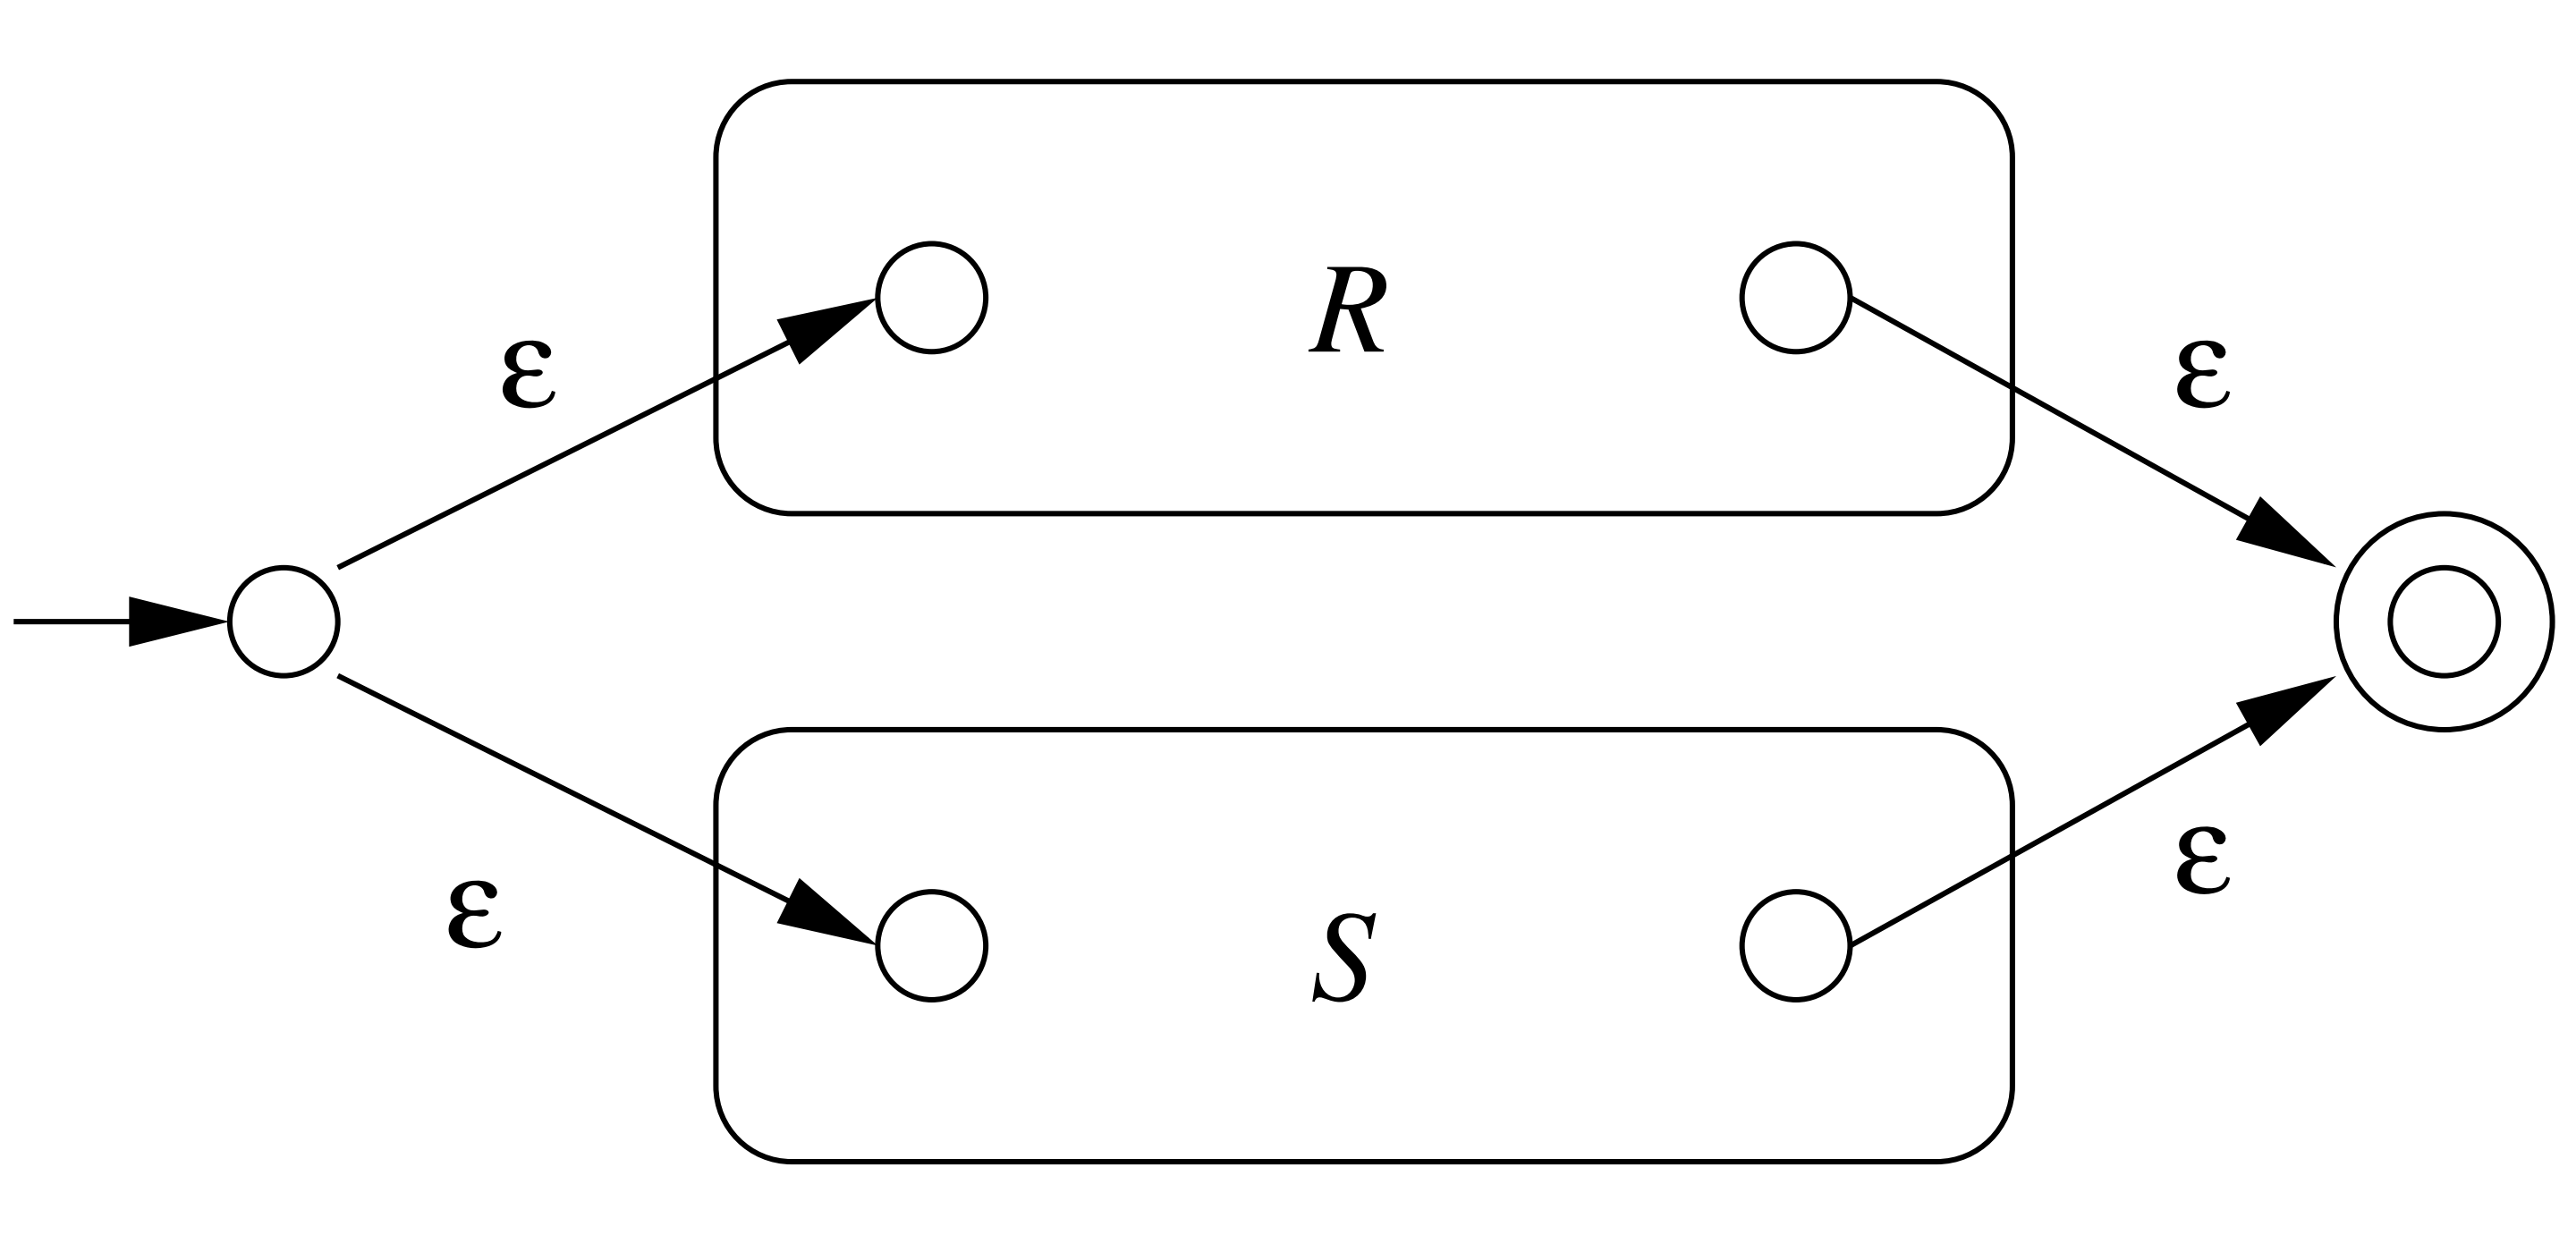
\includegraphics[scale=0.07]{assets/unione.png}
\subsubsection*{Concatenazione}
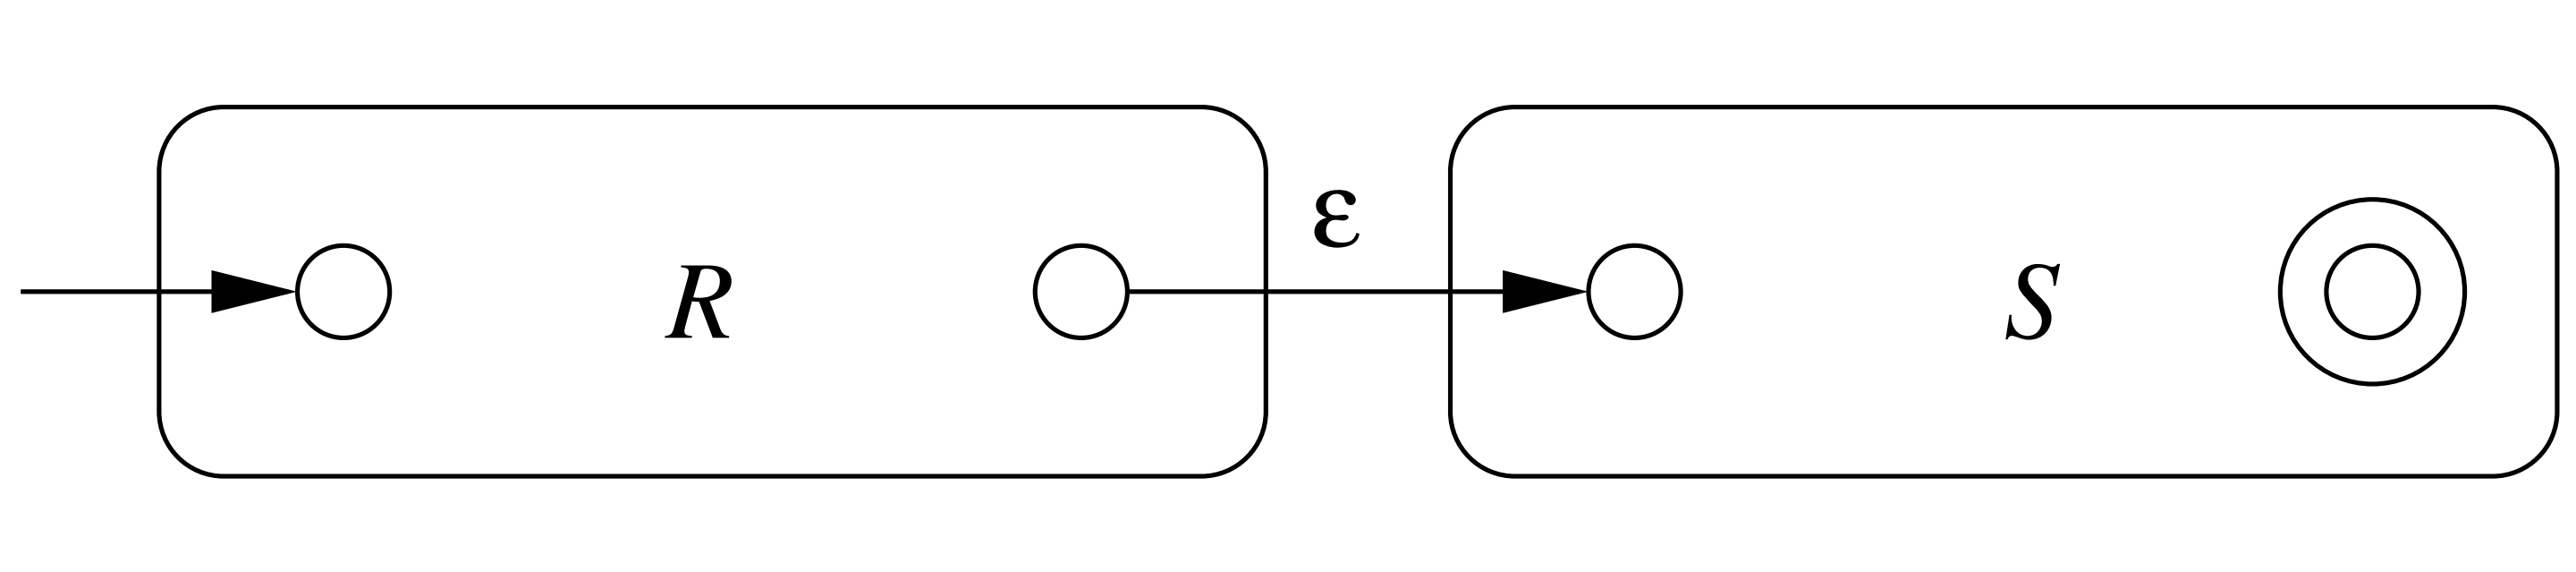
\includegraphics[scale=0.07]{assets/concatenazione.png}
\subsubsection*{Chiusura}
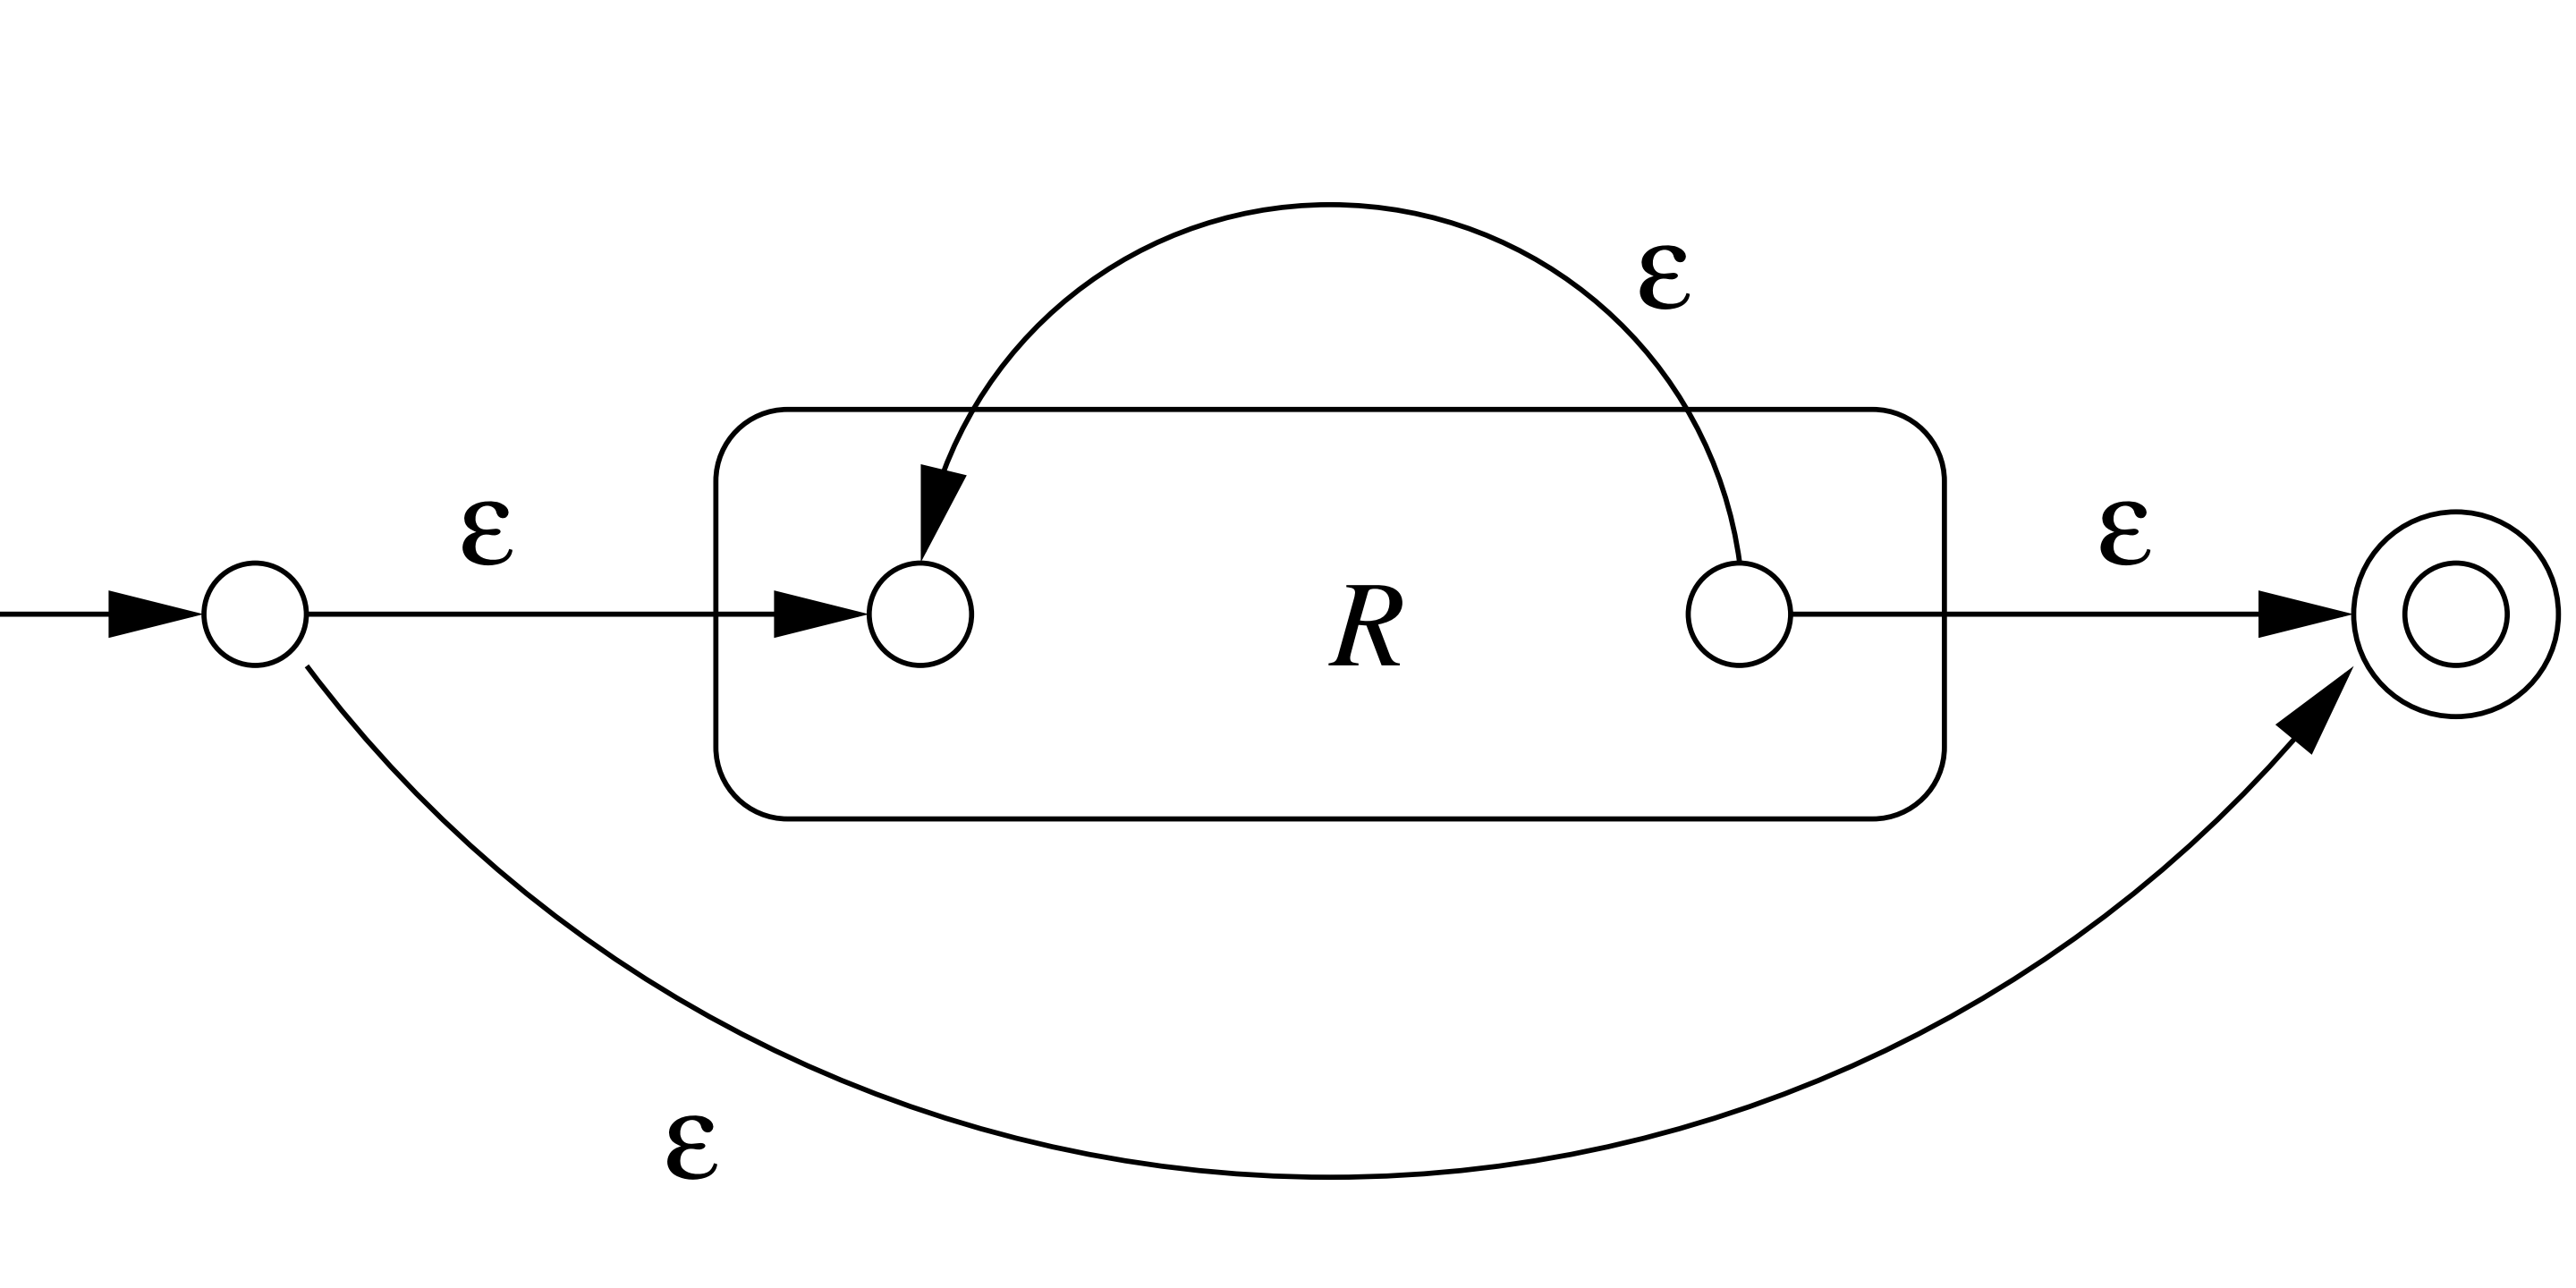
\includegraphics[scale=0.07]{assets/chiusura.png}

\subsubsection{Pumping Lemma}

Sia $L$ un linguaggio regolare.\\
Allora $\exists n$, che dipende solo dal linguaggio, tale che $\forall w \in L,\ |w| \ge n, w$ si può scrivere come la concatenazione di tre  sottostringhe $xyz$ tali che:
\begin{gather*}
    y\neq \epsilon\\
    |xy| \leq n \\
    \forall k \geq 0,\ xy^kz \in L
\end{gather*}

\section{Grammatiche}
\subsection{Derivazioni di una Grammatica}
La Grammatica è una quadrupla $(V,T,P,S)$:
\begin{itemize}
    \item $V$: insieme delle \textbf{variabili} o \textbf{non terminali}
    \item $T$: insieme dei \textbf{terminali}
    \item $P$: insieme delle \textbf{produzioni} o \textbf{regole di riscrittura}
    \item $S$: il simbolo \textbf{iniziale} o \textbf{assioma}. Da questo si parte, e con le regole, si generano le stringhe che formeranno il linguaggio.
\end{itemize}
Seguendo queste regole si generano delle stringhe che formano un linguaggio.
\begin{itemize}
    \item[Esempio] Consideriamo le seguente grammatica $G_1$
    \begin{equation*}
        G_1=(\{S,A\},\{a,b\},S,\{S \implies aAb,aA \implies aaAb,A\implies \epsilon\})
    \end{equation*}
    \begin{align*}
        S &\implies \underline{aA}b\\
        &\implies a\underline{aA}bb\\
        &\implies aaa\underline{A}bbb\\
        &\implies aaabbb
    \end{align*}
\end{itemize}

\subsection{Grammatiche Context-Free}
La Grammatica Context-Free è una quadrupla $(V,\Sigma,P,S)$:
\begin{itemize}
    \item $V$: insieme delle \textbf{variabili} o \textbf{non terminali}
    \item $\Sigma$: insieme dei \textbf{terminali}
    \item $P$: insieme delle \textbf{produzioni} o \textbf{regole di riscrittura}
    \item $S$: il simbolo \textbf{iniziale} o \textbf{assioma}. Da questo si parte, e con le regole, si generano le stringhe che formeranno il linguaggio.
\end{itemize}
La \textbf{quadrupla} contiene queste regole che, seguite, generano delle stringhe.\\
L'insieme di queste \textbf{stringhe} formano il \textbf{linguaggio} $L$ generato dalla grammatica $G$:
\begin{equation*}
    L(G)
\end{equation*}

\subsection{Alberi Sintattici}
Un albero è un \textbf{albero sintattico} se:
\begin{itemize}
    \item Ogni nodo interno è etichettato con una \textbf{variabile $V$}.
    \item Ogni foglia è etichettata con un simbolo in $V \cup T \cup \{\epsilon\}$.
\end{itemize}
Il \textbf{prodotto} di un albero sintattico è la stringa di foglie da \textbf{sinistra a destra}.\\
Le derivazioni possono essere:
\begin{itemize}
    \item Leftmost - si espandono per prima le \textbf{variabili} più a sinistra.
    \item Rightmost - si espandono per prima le \textbf{variabili} più a destra.
\end{itemize}
Una Grammatica si dice \textbf{ambigua} se esiste \textbf{almeno una} stringa che abbia \textbf{due o più alberi} sintattici.

\subsection{Automi a Pila - Pushdown Automata (PDA)}
Un \textbf{PDA} è un modo per implementare una Context-Free Grammar in un modo simile in cui implementiamo un \textbf{Linguaggio Regolare} usando gli \textbf{Automi a Stati Finiti}.\\
Essi hanno \textbf{più memoria} grazie allo \textbf{stack}.\\
Un PDA ha 3 componenti:
\begin{itemize}
    \item Input - stringa di input
    \item Finite Control Unit - in base all'input fa la \textbf{PUSH} o \textbf{POP} dallo \textbf{stack}
    \item Stack (con memoria infinita)
\end{itemize}
\textbf{PDA} è una tupla di 7 elementi:
\begin{equation*}
    P=(Q,\Sigma,\Gamma,\delta,q_0,Z_0,F)
\end{equation*}
dove
\begin{itemize}
    \item $Q$ è un insieme finito di stati
    \item $\Sigma$ è un alfabeto finito di input
    \item $\Gamma$ è un alfabeto finito di pila
    \item $\delta$ è la funzione di transizione
    \item $q_0$ è lo stato iniziale
    \item $Z_0 \in \Gamma$ è il simbolo iniziale per la pila
    \item $F \subseteq Q$ è l'insieme di stati di accettazione  
\end{itemize}

\subsubsection{Diagrammi di transizione}
Un PDA può essere rappresentato da un diagramma di transizione in cui le etichette
sono della forma
\begin{equation*}
    a,X/\gamma
\end{equation*}
in cui
\begin{itemize}
    \item $a$ è il simbolo di \textbf{input}
    \item $X$ è la \textbf{cima della pila}
    \item $\gamma$ è la stringa che sostituisce $X$ sulla pila
\end{itemize}

\subsubsection{Descrizioni istantanee}
Un PDA passa da una configurazione ad un’altra
configurazione consumando un simbolo di input usando le \textbf{descrizioni istantanee} (ID) del PDA. 
Una ID e’ una tripla $(q, w, \gamma)$ dove
\begin{itemize}
    \item $q$ è lo stato in cui si trova l'automa
    \item $w$ è l'input rimanente (es. 0010). Lettura da sinistra a destra.
    \item $\gamma$ è il contenuto della pila (es. $ZZZ_0$)
\end{itemize}

\subsubsection{Da CFG a PDA}
Sia $G=(V,T,Q,S)$ una CFG. Definiamo $P_G$ come
\begin{equation*}
    (\{q\},T,V \cup T,\delta,q,S)
\end{equation*}
dove
\begin{equation*}
    \delta(q,\epsilon A) = \{(q,\beta)\ :\ A \rightarrow \beta \in Q\}
\end{equation*}
per $A \in V$, e
\begin{equation*}
    \delta(q,a,a)=\{(q,\epsilon)\}
\end{equation*}
per $a \in T$.\\
Example
\begin{equation*}
    S \rightarrow aSbS\ |\ bSaS\ |\ \epsilon
\end{equation*}
è definito da
\begin{align*}
    &\delta(q,\epsilon,S)=\{(q,aSbS),(q,bSaS),(q,\epsilon)\}\\
    &\delta(q,a,a)=\{(q,\epsilon)\}\\
    &\delta(q,b,b)=\{(q,\epsilon)\}\\
\end{align*}
per esempio:
\begin{align*}
    (q,ab,S)\vdash(q,ab,aSbS)\vdash(q,b,SbS)\vdash(q,b,bS)\vdash(q,\epsilon,S)\vdash(q,\epsilon,\epsilon)
\end{align*}

\subsection{$FIRST$}
Data una grammatica e una \textbf{stringa} $\alpha$.\\
$FIRST(\alpha)$ è l'insieme dei \textbf{terminali} con cui \textit{iniziano} le stringhe derivabili dalla stringa data ($\alpha$).\\
Formalmente:
\begin{equation*}
    FIRST(\alpha) = \{a\ |\ \alpha \rightarrow^*a\beta\} \cup \{\epsilon\ |\ se\  \alpha \rightarrow^*\epsilon\}
\end{equation*}
\begin{enumerate}
    \item se $X$ è un simbolo \textbf{terminale} (lettera minuscola) allora $FIRST(X)=X$.
    \item se $X \implies \epsilon$ è una \textbf{produzione} allora \textbf{aggiungi} $FIRST(X)=\{\epsilon\}$.
    \item se $X$ è un \textbf{non-terminale} e $X \implies Y_1,Y_2\dots Y_K$ è una \textbf{produzione} allora \textbf{aggiungi} $FIRST(Y_1)$ al $FIRST(X)$\\
            se $Y_1 \implies \epsilon$ (deriva $\epsilon$) allora \textbf{aggiungi} $FIRST(Y_2)$ al $FIRST(X)$.
\end{enumerate}

\subsection{$FOLLOW$}
Data una grammatica e una \textbf{variabile} $A$.\\
$FOLLOW(A)$(insieme dei \textbf{seguiti}) è l'insieme dei terminali con cui \textit{iniziano} le stringhe che seguono $A$ nelle derivazioni.\\
Formalmente:
\begin{equation*}
    FOLLOW(A)=\{a\ |\ S \rightarrow^* \alpha Aa\beta\} \cup \{\$\ |\ se\ S \rightarrow^*\alpha A\}
\end{equation*}
\begin{enumerate}
    \item se $X$ è il \textbf{simbolo di start} allora $FOLLOW(X)=\$$.
    \item se $A \implies \alpha B \beta$ è una \textbf{produzione} allora $FOLLOW(B)=FIRST(\beta)$ eccetto $\epsilon$, se $B$ contiene $\epsilon$.
    \item se $A \implies \alpha B \beta$ o $A \implies \alpha B \beta$ e $FIRST(\beta)$ contiene $\epsilon$ allora \textbf{aggiungi} $FOLLOW(A)$ al $FOLLOW(B)$.
\end{enumerate}

\subsection{Insieme Guida}
L'\textbf{Insieme Guida} di una produzione (es. $A \rightarrow \alpha$) indica l'\textbf{insieme dei TERMINALI} con cui iniziano le stringhe generabili partendo dalla produzione stessa (\$ se ci si trova alla fine della parola).\\
Sostanzialmente serve a capire quali sono le \textbf{iniziali} (terminali, ad es. $a,b,c,\dots$) delle stringhe che si possono generare da una specifica produzione.
\begin{itemize}
    \item $GUI(A \rightarrow \alpha) \implies FIRST(\alpha)$ oppure
    \item $GUI(A \rightarrow \alpha) \implies FIRST(\alpha)\cup FOLLOW(A)$ se $\epsilon$ appartiene al $FIRST(\alpha)$
\end{itemize}

\newpage

\begin{table}
    \centering
    \begin{tabular}{|l|c|c|}
                        & $FIRST$         & $FOLLOW$     \\
    $S \implies ABCDE$     & $\{a,b,c\}$     & $\{\$\}$     \\
    $A \implies a\ |\ \epsilon$ & $\{a,\epsilon\}$ & $\{b,c\}$    \\
    $B \implies b\ |\ \epsilon$ & $\{b,\epsilon\}$ & $\{c\}$      \\
    $C \implies c$         & $\{c\}$         & $\{d,e,\$\}$ \\
    $D \implies d\ |\ \epsilon$ & $\{d,\epsilon\}$ & $\{e,\$\}$   \\
    $E \implies e\ |\ \epsilon$ & $\{e,\epsilon\}$ & $\{\$\}$    
    \end{tabular}
\end{table}

\subsection{Parser $LL(1)$}
\subsection{Proprietà principali delle Grammatiche $LL(1)$}
\begin{itemize}
    \item Non ambigua (esiste solo una derivazione left-most)
    \item Assenza di Ricorsioni Sinistre
\end{itemize}
\subsubsection{Ricorsioni Sinistre}
Si ha una \textbf{Ricorsione Sinistra} quando una variabile \textit{chiama} se stessa 
\begin{equation*}
    S \implies S\alpha
\end{equation*}
questo non è gestibile da un Parser Top-Down. Una produzione del seguente tipo
\begin{equation*}
    A \implies A\alpha_1\ |\ \dots\ |\ A\alpha_n\ |\ \beta_1\ |\ \dots\ |\ \beta_m
\end{equation*}
(le stringhe $\beta_i$ non iniziano con $A$)\\
si può sostituire con una \textbf{fattorizzazione destra} in questo modo
\begin{equation*}
    \begin{aligned}
        A &\implies \beta_1A'\ |\ \dots\ |\ \beta_mA'\\        
        A' &\implies \epsilon\ |\ \alpha_1A'\ |\ \dots\ |\ \alpha_nA'
    \end{aligned}
\end{equation*}

\subsubsection{Fattorizzazione Sinistra}
Si ha una \textbf{Fattorizzazione Sinistra} quando una variabile ha multiple produzioni con lo stesso prefisso
\begin{equation*}
    A \implies \textbf{ab}c\ |\ \textbf{ab}\ |\ \textbf{ab}b
\end{equation*}
e si risolve così
\begin{equation*}
    \begin{aligned}
        A &\implies \textbf{ab}A'\\
        A' &\implies c\ |\ \epsilon\ |\ b
    \end{aligned}
\end{equation*}

\subsection{Analizzatore a Discesa Ricorsiva}
Ad ogni variabile $A$ con produzioni
\begin{equation*}
    \begin{aligned}
        A \rightarrow \alpha_1\\
        A \rightarrow \alpha_2\\
        \dots\\
        A \rightarrow \alpha_k
    \end{aligned}
\end{equation*}

si associa una procedura:
\begin{lstlisting}[escapeinside={*}{*}]
    function A()
        if (cc *$\in GUI(A \rightarrow \alpha_1)$*)
            body *$(\alpha_1)$*
        else if (cc *$\in GUI(A \rightarrow \alpha_a)$*)
            body *$(\alpha_a)$*
        *\dots*
        else if (cc *$\in GUI(A \rightarrow \alpha_k)$*)
            body *$(\alpha_k)$*
        else ERRORE (*\dots*)
\end{lstlisting}

\section{Traduzione Diretta della Sintassi}
\subsection{Attributi Ereditati o Sintetizzati}
\subparagraph*{Sintetizzati}
Un attributo sintetizzato per una variabile $A$ in un nodo $n$ dell’albero di parsificazione 
è definito da una regola semantica associata alla produzione in $n$, e il suo valore è calcolato
solo in termini dei valori degli attributi nei nodi figli di $n$ ed in $n$ stesso. ($A$ è il simbolo a sinistra nella produzione).
\begin{equation*}
    E \rightarrow E_1 + T\  \{E.val = E_1.val + T.val\}
\end{equation*}
\subparagraph*{Ereditati}
Un attributo ereditato per una variabile $A$ in un nodo $n$ dell’albero di parsificazione è definito
da una regola semantica associata alla produzione nel nodo padre di $n$ e il suo valore è calcolato
solo in termini dei valori degli attributi del padre di $n$, di $n$ stesso e dei suoi fratelli. 
($A$ è un simbolo nel corpo della produzione, cioè al membro  destro).
\begin{equation*}
    A \rightarrow BCD \{ C.in = A.in,\ C.type = B.type \} 
\end{equation*}

\subsection{Definizioni $S$-attribuite ed $L$-attribuite}
\subparagraph*{$S$-attribuite}
Una \textbf{SDD} è $S$-attribuita se tutti gli attributi sono sintetizzati.
\subparagraph*{$L$-attribuite}
Una \textbf{SDD} è $L$-attribuita se gli attribuiti sono:
\begin{itemize}
    \item \textbf{sintetizzati} oppure
    \item \textbf{ereditati} e soddisfano il seguente vincolo:\\
    per ogni produzione $A \rightarrow X_1, X_2, \dots, X_n$ ogni attributo ereditato di $X_j$ dipende solo da:
    \begin{itemize}
        \item attributi ereditati o sintetizzati dei simboli $X_1,X_2, \dots, X_{j-1}$ a sinistra di $X_j$ nella produzione
        \item attributi ereditati di $A$
        \item attributi ereditati o sintetizzati di $X_j$ purché non vi siano cicli nel grafo delle dipendenze formati dagli attributi di questa occorrenza di $X_j$.
        \\ \textbf{Cioè nel grafo delle dipendenze gli archi tra gli attributi associati a una produzione possono andare da sinistra a destra, ma non da destra a sinistra.}
    \end{itemize}
\end{itemize}
Esempio:
\begin{align*}
   &P_1:\ S \rightarrow MN\ \{S.val= M.val + N.val\}\\
   &P_2:\ M \rightarrow PQ\ \{M.val = P.val * Q.val\  and\ P.val =Q.val\} 
\end{align*}
$P_1$ è $L$-attribuita, invece $P_2$ non lo è.\\
In $P_1$, $S$ è un attributo \textbf{sintetizzato} e nelle definizioni 
$L$-attribuite è permesso.\\ 
Invece $P_2$ non rispetta la definizione $L$-attribuita  
siccome $P$ dipende da $Q$ che è alla sua \textbf{destra}.
\newpage


\section{DOMANDE}
\subsection{Quando una grammatica è LL(1)?}
Se per ogni coppia di produzioni a partire da uno stesso simbolo non terminale $A:\\
A\implies \alpha$ e $A \implies \beta$, si ha\\
$GUI(A \implies \alpha) \cap GUI(A \implies \beta) = \Phi$.\\
Ovvero, gli \textbf{insiemi guida} $GUI()$ di un simbolo con due produzioni distinte non coincidono (non hanno elementi in comune).

\subsection{Cosa è un linguaggio regolare? Come si verifica?}
\subsection{Differenza tra linguaggi Context-Free e non? Come lo stabilisco?}
Regular grammar is either right or left linear, whereas context free grammar is basically any combination of terminals and non-terminals. 
Hence you can see that regular grammar is a subset of context-free grammar.
\subsection{Quando una grammatica è ambigua?}
Una grammatica è ambigua se almeno una frase del linguaggio generato è ambigua.\\
Una frase è ambigua se ha almeno due \textbf{alberi sintattici} distinti.
\subsection{Completare la definizione della funzione di transizione $\sigma_D$ dell'automa a stati finiti deterministico}
\subsection{Quando due stati $p$ e $q$ sono indistinguibili? E i-indistinguibili?}
Sono i-indistinguibili se e solo se nessuna stringa di lunghezza $\le i$ distingue $p$ da $q$.\\
Sono indistinguibili se e solo se nessuna stringa (di qualunque lunghezza) distingue $p$ da $q$.
\subsection{Due stati i-indistinguibili quando sono i+1-distinguibili?}
Questo si verifica quando con la stessa stringa di input i due stati raggiunti appartengono a due sottoinsiemi diversi dalla Partizione i ($\Pi_i$)
\subsection{Quando un automa è minimo?}
Un automa è minimo quando la partizione degli stati contiene i gruppi degli stati indistinguibili.
\subsection{Quando una grammatica è LL(1)?}
Una grammatica è $LL(1)$ se per ogni non terminale $A$ e per ogni coppia di produzioni
\begin{align*}
    A &\rightarrow \alpha\\
    A &\rightarrow \beta
\end{align*}
gli insiemi guida sono disgiunti:
\begin{align*}
    GUI(A \rightarrow \alpha) \cap GUI(A \rightarrow \beta) = \Phi
\end{align*}
Una grammatica \textbf{non può essere} $LL(1)$ se è \textbf{ricorsiva sinistra}.\\
Perché l'intersezione degli
insiemi $GUI$ delle produzioni sono uguali.
\subsection{Differenza tra SDD S-attribuiti e l-attribuiti}
\begin{itemize}
    \item $S-$attribuiti tutti gli attribuiti sono sintetizzati
    \item $L-$attribuiti gli attribuiti possono essere sia sintetizzati che ereditati, ereditati con le seguenti regole:
    \begin{itemize}
        \item pagina 29/36 di 4/22-traduzione1.pdf
    \end{itemize}
\end{itemize}
\subsection{MEMO}
\textbf{I Linguaggi Regolari sono sottoinsiemi dei CFG (Context Free Grammar)}.\\
Linguaggi context free (generati da CFG) riconosciuti da
\begin{itemize}
    \item PDA
    \item NPDA
\end{itemize}
Linguaggi regolari riconosciuiti da
\begin{itemize}
    \item DFA
    \item NFA
    \item $\epsilon$-NFA % 
    \smash{\raisebox{.3\dimexpr3\baselineskip+6\itemsep+2\parskip}{$\left.\rule{0pt}{.5\dimexpr3\baselineskip+3\itemsep+3\parskip}\right\}\text{Riconoscono linguaggi regolari}$}}
  \end{itemize}
\subparagraph*{Minimizzazione Automi}
Per Minimizzare NFA occorre prima convertirli in DFA e poi minimizzare il DFA.

\section{Domande PDF}
\subsection{Parte I}

\newcommand\Que[1]{%
   \leavevmode\par
   \stepcounter{question}
   \noindent
   \thequestion. \textbf{#1}\par}

\newcommand\Ans[2][]{%
    \leavevmode\par\noindent
   {\leftskip37pt
    \textbf{#1}#2\par}}

    \Que{ Cos'è un alfabeto?}
    \Ans{Un insieme di simboli con cui comporre stringhe}
    \Que{ Cos'è una stringa?}
    \Ans{Un'insieme di simboli (tra quelli dell'alfabeto) che rispetta le regole di costruzione di una certe grammatica}
    \Que{ Quando due stringhe sono uguali?}
    \Ans{Se i loro caratteri, letti ordinatamente da sx a dx, coincidono.}
    \Que{ Cos'è una sottostringa?}
    \Ans{La stringa $Y$ è una sottostringa della stringa $X$ se esistono delle stringhe $U$ e $V$ tali che\\
    $X = UYV$}
    \Que{ Cos'è un prefisso?}
    \Ans{La stringa Y è un prefisso della stringa X se esiste una stringa $V$ tale che $X = YV$}
    \Que{ Cos'è un suffisso?}
    \Ans{La stringa Y è un suffisso della stringa X se esiste una stringa $U$ tale che $X = UY$}
    \Que{ Cos'è la concatenazione? Quali proprietà ha?}
    \Ans{La concatenazione di due stringhe è la stringa formata dai simboli della prima stringa seguiti da quelli della seconda.\\
    \begin{itemize}
        \item NON è commutativa
        \item E' associativa
        \item HA un ELEMENTO NEUTRO
        \item la lunghezza della stringa concatenazione è la somma delle lunghezze delle due stringhe.
    \end{itemize}}
    \Que{ Cos'è la riflessione? Quali proprietà ha?}
    \Ans{La riflessione è la stringa ottenuta scrivendo i caratteri in ordine inverso.\\
    Il riflesso del riflesso  di una stringa è la stringa stessa\\
    La riflessione della concatenazione di due stringhe è la concatenazione inversa delle loro riflessioni.\\
    La riflessione della stringa vuota è la stringa vuota\\
    La riflessione ha la precedenza sul concatenamento.}
    \Que{ Cos'è la potenza?}
    \Ans{La potenza n-esima della stringa $X$ è il concatenamento di $X$ con se stessa $n$ volte.}
    \Que{Cos'è un linguaggio?}
    \Ans{Un linguaggio è un insieme di stringhe su quell'alfabeto}
    \Que{Cos'è l'insieme dei prefissi?}
    
    \Que{ Quando un linguaggio è privo di prefissi?}
    \Ans{Se non contiene i prefissi delle sue stringhe.\\
        $L \cap$ Prefissi $(L) = \Phi$}
    \Que{ Cosa sono la riflessione, la concatenazione e la potenza di un linguaggio?}
    \Ans{
    \begin{itemize}
        \item La riflessione di un linguaggio $L$ è l'insieme delle stringhe riflesse di $L$
        \item La concatenazione di  due linguaggi $L1$ e $L2$ è l'insieme ottenuto concatenando in tutti i modi possibili le stringhe di $L1$ con le stringhe di $L2$
        \item La potenza n-esima di un linguaggio $L$ è il concatenamento di $L$ con se stesso $n$ volte.
    \end{itemize}}    
    \Que{ Cos'è la chiusura di Kleene di un linguaggio $L$? Quali proprietà ha?}
    \Ans{E' l'unione di tutte le potenze di $L$.\\
    Le proprietà:
    \begin{itemize}
        \item monotonia
        \item chiusura rispetto al concatenamento
        \item idempotenza
        \item commutatività della riflessione con la chiusura di Kleene e con la potenza.
    \end{itemize}}
    \Que{ Che cos'è la chiusura non riflessiva?}
    \Ans{E' l'unione di tutte le potenze positive di $L$}
    \Que{ Che cos'è il linguaggio universale su un alfabeto $\Sigma$ ?}
    \Ans{E' la sua chiusura di Kleene.}
    \Que{ Che cos'è il complemento di un linguaggio $L$ su un alfabeto $\Sigma$   rispetto ad un alfabeto $\Delta$?}
        \Ans{E' la differenza tra $\Delta^*$ ed L}


\subsection{Parte II}


\end{document}